\begin{figure}[ht!]
    \centering
    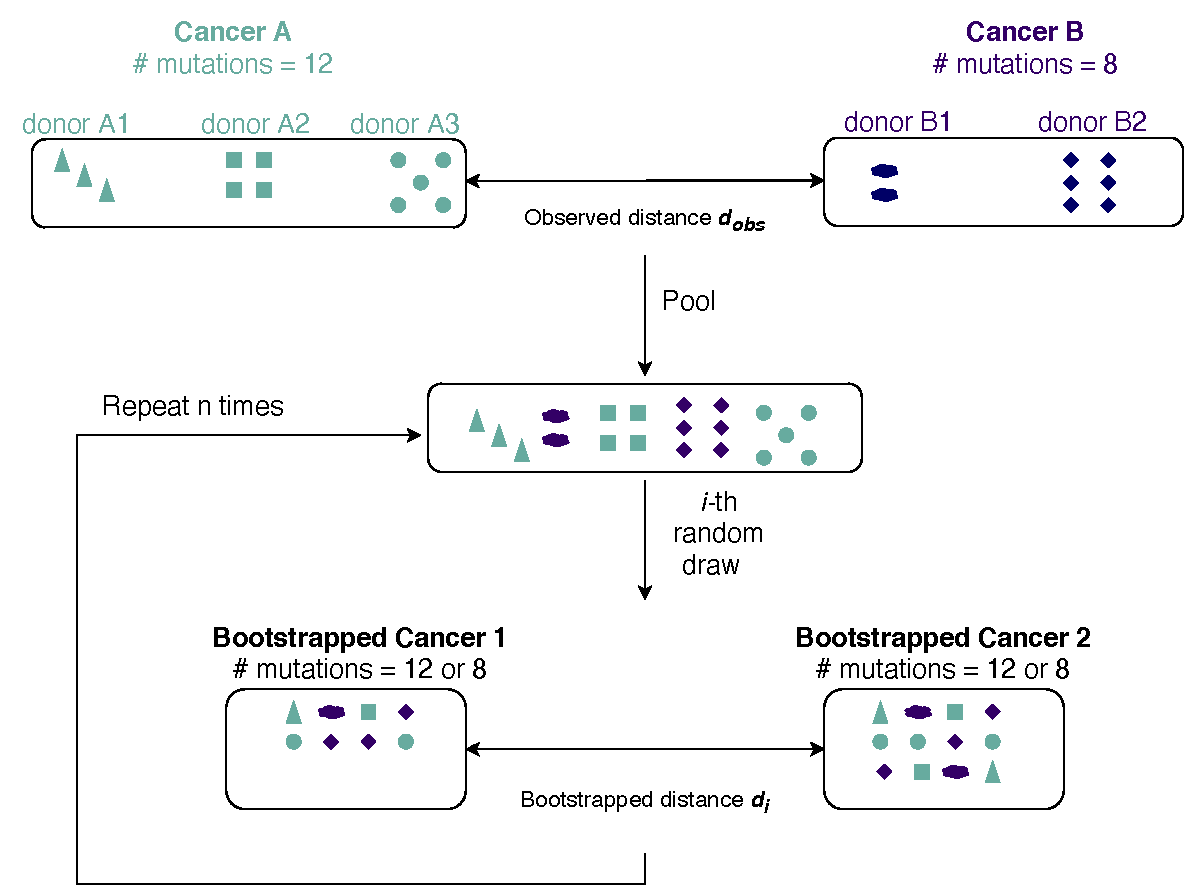
\includegraphics[scale=0.6]{graphics/bootstrap_demo.pdf}
    \caption{\textbf{Testing the hypothesis that two cancers share the same genomic distribution of mutations using bootstrap.} Mutations are pooled from 2 original cancers A and B, the distance between A and B is $d_{obs}$. Two bootstrapped cancers 1 and 2 are then simulated by randomly drawing mutations from the pool, the number of mutations in 1 and 2 must be the same as either A or B. The distance $d_i$ between cancers 1 and 2 is then measured. This process is repeated 1000 times for each of the representations introduced. The estimated p-value is the number of times $d_i \geqslant d_{obs}$ divided by $n$.}
    \label{fig:bootstrap_demo}
\end{figure}
